\begin{pages}
    \begin{Rightside}
    \selectlanguage{greek}
        \beginnumbering
        \pstart[
        			\chapter{Αἱ ἐπιστολαὶ ταῖς ἐν Ἐφέσῳ, Σμύρνῃ, Περγάμῳ καὶ Θυατείροις ἐκκλησίαις}
        			\markboth{Letters to the Churches in Ephesus, Smyrna, Pergamum and Thyatira}
				]
			Τῷ ἀγγέλῳ τῆς ἐν Ἐφέσῳ ἐκκλησίας γράψον Τάδε λέγει ὁ κρατῶν τοὺς ἑπτὰ ἀστέρας ἐν τῇ δεξιᾷ αὐτοῦ, ὁ περιπατῶν ἐν μέσῳ τῶν ἑπτὰ λυχνιῶν τῶν χρυσῶν Οἶδα τὰ ἔργα σου καὶ τὸν κόπον καὶ τὴν ὑπομονήν σου, καὶ ὅτι οὐ δύνῃ βαστάσαι κακούς, καὶ ἐπείρασας τοὺς λέγοντας ἑαυτοὺς ἀποστόλους καὶ οὐκ εἰσίν, καὶ εὗρες αὐτοὺς ψευδεῖς· καὶ ὑπομονὴν ἔχεις, καὶ ἐβάστασας διὰ τὸ ὄνομά μου, καὶ οὐ κεκοπίακες. 
		\pend 
		\pstart
			ἀλλὰ ἔχω κατὰ σοῦ ὅτι τὴν ἀγάπην σου τὴν πρώτην ἀφῆκες. μνημόνευε οὖν πόθεν πέπτωκες, καὶ μετανόησον καὶ τὰ πρῶτα ἔργα ποίησον· εἰ δὲ μή, ἔρχομαί σοι καὶ κινήσω τὴν λυχνίαν σου ἐκ τοῦ τόπου αὐτῆς, ἐὰν μὴ μετανοήσῃς.
		\pend
		\pstart
			ἀλλὰ τοῦτο ἔχεις, ὅτι μισεῖς τὰ ἔργα τῶν Νικολαϊτῶν, ἃ κἀγὼ μισῶ. Ὁ ἔχων οὖς ἀκουσάτω τί τὸ Πνεῦμα λέγει ταῖς ἐκκλησίαις. Τῷ νικῶντι δώσω αὐτῷ φαγεῖν ἐκ τοῦ ξύλου τῆς ζωῆς, ὅ ἐστιν ἐν τῷ Παραδείσῳ τοῦ Θεοῦ.
		\pend
		\pstart
			Καὶ τῷ ἀγγέλῳ τῆς ἐν Σμύρνῃ ἐκκλησίας γράψον Τάδε λέγει ὁ πρῶτος καὶ ὁ ἔσχατος, ὃς ἐγένετο νεκρὸς καὶ ἔζησεν Οἶδά σου τὴν θλῖψιν καὶ τὴν πτωχείαν, ἀλλὰ πλούσιος εἶ, καὶ τὴν βλασφημίαν ἐκ τῶν λεγόντων Ἰουδαίους εἶναι ἑαυτούς, καὶ οὐκ εἰσίν ἀλλὰ συναγωγὴ τοῦ Σατανᾶ. μὴ φοβοῦ ἃ μέλλεις πάσχειν. ἰδοὺ μέλλει βάλλειν ὁ διάβολος ἐξ ὑμῶν εἰς φυλακὴν ἵνα πειρασθῆτε, καὶ ἕξετε θλῖψιν ἡμερῶν δέκα. γίνου πιστὸς ἄχρι θανάτου, καὶ δώσω σοι τὸν στέφανον τῆς ζωῆς. Ὁ ἔχων οὖς ἀκουσάτω τί τὸ Πνεῦμα λέγει ταῖς ἐκκλησίαις. Ὁ νικῶν οὐ μὴ ἀδικηθῇ ἐκ τοῦ θανάτου τοῦ δευτέρου.
		\pend
		\pstart
			Καὶ τῷ ἀγγέλῳ τῆς ἐν Περγάμῳ ἐκκλησίας γράψον Τάδε λέγει ὁ ἔχων τὴν ῥομφαίαν τὴν δίστομον τὴν ὀξεῖαν Οἶδα ποῦ κατοικεῖς· ὅπου ὁ θρόνος τοῦ Σατανᾶ· καὶ κρατεῖς τὸ ὄνομά μου, καὶ οὐκ ἠρνήσω τὴν πίστιν μου καὶ ἐν ταῖς ἡμέραις Ἀντιπᾶς ὁ μάρτυς μου ὁ πιστός μου, ὃς ἀπεκτάνθη παρ’ ὑμῖν, ὅπου ὁ Σατανᾶς κατοικεῖ.
		\pend
		\pstart	
			ἀλλ’ ἔχω κατὰ σοῦ ὀλίγα, ὅτι ἔχεις ἐκεῖ κρατοῦντας τὴν διδαχὴν Βαλαάμ, ὃς ἐδίδασκεν τῷ Βαλὰκ βαλεῖν σκάνδαλον ἐνώπιον τῶν υἱῶν Ἰσραήλ, φαγεῖν εἰδωλόθυτα καὶ πορνεῦσαι. οὕτως ἔχεις καὶ σὺ κρατοῦντας τὴν διδαχὴν τῶν Νικολαϊτῶν ὁμοίως. μετανόησον οὖν· εἰ δὲ μή, ἔρχομαί σοι ταχύ καὶ πολεμήσω μετ’ αὐτῶν ἐν τῇ ῥομφαίᾳ τοῦ στόματός μου. Ὁ ἔχων οὖς ἀκουσάτω τί τὸ Πνεῦμα λέγει ταῖς ἐκκλησίαις. Τῷ νικῶντι δώσω αὐτῷ τοῦ μάννα τοῦ κεκρυμμένου, καὶ δώσω αὐτῷ ψῆφον λευκήν, καὶ ἐπὶ τὴν ψῆφον ὄνομα καινὸν γεγραμμένον, ὃ οὐδεὶς οἶδεν εἰ μὴ ὁ λαμβάνων.
		\pend
		\pstart
			Καὶ τῷ ἀγγέλῳ τῆς ἐν Θυατείροις ἐκκλησίας γράψον Τάδε λέγει ὁ Υἱὸς τοῦ Θεοῦ, ὁ ἔχων τοὺς ὀφθαλμοὺς αὐτοῦ ὡς φλόγα πυρός, καὶ οἱ πόδες αὐτοῦ ὅμοιοι χαλκολιβάνῳ Οἶδά σου τὰ ἔργα καὶ τὴν ἀγάπην καὶ τὴν πίστιν καὶ τὴν διακονίαν καὶ τὴν ὑπομονήν σου, καὶ τὰ ἔργα σου τὰ ἔσχατα πλείονα τῶν πρώτων. 
		\pend
		\pstart
			ἀλλὰ ἔχω κατὰ σοῦ ὅτι ἀφεῖς τὴν γυναῖκα Ἰεζάβελ, ἡ λέγουσα ἑαυτὴν προφῆτιν, καὶ διδάσκει καὶ πλανᾷ τοὺς ἐμοὺς δούλους πορνεῦσαι καὶ φαγεῖν εἰδωλόθυτα· καὶ ἔδωκα αὐτῇ χρόνον ἵνα μετανοήσῃ, καὶ οὐ θέλει μετανοῆσαι ἐκ τῆς πορνείας αὐτῆς.
		\pend
		\pstart	
			ἰδοὺ βάλλω αὐτὴν εἰς κλίνην, καὶ τοὺς μοιχεύοντας μετ’ αὐτῆς εἰς θλῖψιν μεγάλην, ἐὰν μὴ μετανοήσουσιν ἐκ τῶν ἔργων αὐτῆς· καὶ τὰ τέκνα αὐτῆς ἀποκτενῶ ἐν θανάτῳ· καὶ γνώσονται πᾶσαι αἱ ἐκκλησίαι ὅτι ἐγώ εἰμι ὁ ἐραυνῶν νεφροὺς καὶ καρδίας, καὶ δώσω ὑμῖν ἑκάστῳ κατὰ τὰ ἔργα ὑμῶν. ὑμῖν δὲ λέγω τοῖς λοιποῖς τοῖς ἐν Θυατείροις, ὅσοι οὐκ ἔχουσιν τὴν διδαχὴν ταύτην, οἵτινες οὐκ ἔγνωσαν τὰ βαθέα τοῦ Σατανᾶ, ὡς λέγουσιν, οὐ βάλλω ἐφ’ ὑμᾶς ἄλλο βάρος· πλὴν ὃ ἔχετε κρατήσατε ἄχρι οὗ ἂν ἥξω. Καὶ ὁ νικῶν καὶ ὁ τηρῶν ἄχρι τέλους τὰ ἔργα μου, δώσω αὐτῷ ἐξουσίαν ἐπὶ τῶν ἐθνῶν, καὶ ποιμανεῖ αὐτοὺς ἐν ῥάβδῳ σιδηρᾷ, ὡς τὰ σκεύη τὰ κεραμικὰ συντρίβεται, ὡς κἀγὼ εἴληφα παρὰ τοῦ Πατρός μου, καὶ δώσω αὐτῷ τὸν ἀστέρα τὸν πρωϊνόν. Ὁ ἔχων οὖς ἀκουσάτω τί τὸ Πνεῦμα λέγει ταῖς ἐκκλησίαις.
			\pend
        \endnumbering
    \end{Rightside}
    \begin{Leftside}
        \beginnumbering
        \pstart[
        			\chapter{Letters to the Churches in Ephesus, Smyrna, Pergamum and Thyatira}
				]
			To the messenger of the church in Ephesus write (the following): “This is what the One who holds the seven stars in His right hand and who walks amid the seven golden lamp-stands says, ‘I know your works (deeds), your exertion and your patient endurance; and (I know) that you cannot tolerate those who are bad and (I know) that you tested those who claim to be apostles — but are not — and found them to be false. And you have patient endurance and have endured because of (through) my name and you have not grown weary.’ 
		\pend
		\pstart
			‘But what I have against you, is that you left your first love. Remember, then, from where you have fallen and repent (have a change of heart) and do the first works (deeds). If you do not, I will come to you and I will remove your lamp-stand from its place — unless you repent.’
		\pend
		\pstart
			‘But what is in your favour, is that you hate the works (deeds) of the Nicolaitans, which I hate as well. Let him who has ears listen to what the Spirit says to the seven churches. I will give something to eat from the Tree of Live — the one in the paradise of God — to him who is victorious.’”
		\pend
		\pstart
			And to the messenger of the church in Smyrna write (the following): “This is what the First and the Last, the one who died and lived (again), says, ‘I know your suffering and your poverty — even though you are rich — and the slander from those who claim themselves to be Jews — but are not — and are, instead, a synagogue of Satan. Do not be afraid of what you will suffer. Look, the Devil will throw some of you into prison in order for you to be put to the test; and you will have (to endure) suffering for ten days. Be faithful until death, and I will give you the crown of life. Let him who has ears listen to what the Spirit says to the churches. The victor will not be hurt by the second death.’”
		\pend
		\pstart
			And to the messenger of the church in Pergamum write (the following): “This is what the One who has the sharp, double-edged sword says, ‘I know where you live — namely there, where Satan’s throne lies — and (I know that) you hold onto my name; and you did not deny your belief in me, (not) even in the days of Antipas — my faithful witness —, who was killed whilst he was with you — there, where Satan dwells.
		\pend
		\pstart
			‘But I have a few things against you. Namely that you have there those who hold to the teaching of Balaam, who taught Balak to throw a stumbling block before the children of Israel, so that they commit sexual immorality and eat meals offered to idols. You also have those holding to the teaching of the Nicolaitans. Therefore, repent. If not, I will come to you swiftly and fight them with the sword of my mouth. Let him who has ears listen to what the Spirit says to the churches. The victor I will give (something to eat) of the hidden manna and I will give him a white stone; and upon the stone is written a new name, which nobody — except the one who took the stone — knows.’”
		\pend
		\pstart
			And to the messenger of the church in Thyatira write (the following): This is what the Son of God says, who has eyes like a flame of fire and his feet are like brass, ‘I know your works (deeds), your love, your faith, your service, your patient endurance and (that) your last works are greater than the first.
		\pend
		\pstart
			But what I have against you is that you tolerate the woman Isabel, who calls herself a prophetess and teaches and misleads my servants so that they commit sexual immorality and meals offered to idols. And I gave her time to repent and (yet) she does not want to repent of her sexual immorality. 
		\pend	
		\pstart
			Look, I throw her into bed and those who commit adultery with her into great suffering, unless they repent of her deeds. And her children I will kill in death (I will slay them) and every church will know that I am the searcher of thoughts and (of) hearts and I will give to you each according to your deeds. And to you — the remaining (people) of Thyatira, who do not follow (have) this teaching and who did not, as they say, know the deep secrets of Satan — I say, that I will will not throw another burden upon you; hold fast to what you have until I may come. And to the victor and to the one who honours my deeds until the end, I will give (him the) authority over the nations; and he will rule them with an iron rod, and they will be shattered like clay dishes. As I have received from my Father, I, too, will give him (the victor) the Morning Star. Let him who has ears listen to what the Spirit says to the seven churches.’”
		\pend
        \endnumbering
    \end{Leftside}

\end{pages} 
\Pages

\clearpage
\thispagestyle{empty}
\null\vfill
\settowidth\longest{\huge\itshape […] and when I turned around I saw}
\begin{center}
\parbox{\longest}{%
  \raggedright{\huge\itshape%
    ``To the messenger of the church in Ephesus write (the following) […]'' \par\bigskip
  }
  \raggedleft\Large\MakeUppercase{The Angel gives John the Letter for the Church of Ephesus — 1047, Facundus}\par%
}
\vfill\vfill
\clearpage\newpage
\end{center}
\newpage
\thispagestyle{empty}
\begin{center}
	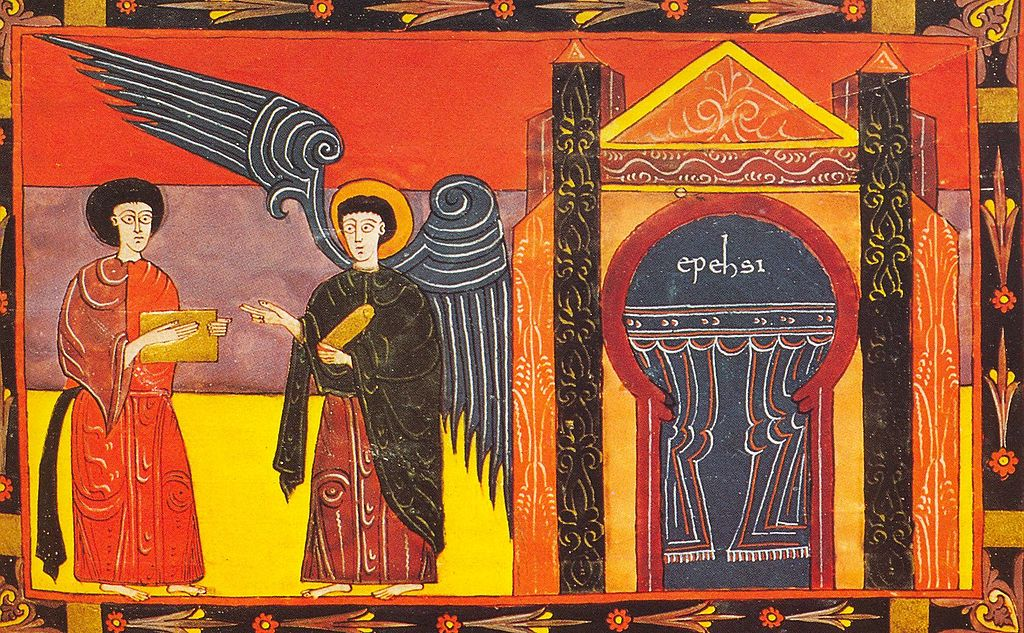
\includegraphics[angle=90, width=0.9\textwidth]{images/illustrations/letterephesus.jpg}
\end{center}